% Document notes:
% Improvements: In Figure 3, make the total voltage table go directly underneath the current table and to the right of the resistor voltage table.
\documentclass [12pt, letterpaper, twoside] {article}
\usepackage[utf8]{inputenc}
\usepackage [left=1.0in, right=1.0in, top=1.0in, bottom=1.0in] {geometry}
% For updated time
\usepackage {datetime}
% For drawing pictures
\usepackage {tikz}
% For equations
\usepackage {amsmath}
% To make tables
\usepackage {tabu}
% For multiple rows in table slot
\usepackage {multirow}
\usepackage {verbatim}
% To add captions
\usepackage {caption}
\usepackage {float}
% To make graphs
\usepackage {pgfplots}
% To make scatter plots
\usepackage{pgfplotstable}
% To make pretty theorems
\usepackage[english]{babel}
% To make circuit drawings
\usepackage{circuitikz}
% To make tables side by side
\usepackage{subfig}

\usetikzlibrary {shapes.geometric, arrows, angles}
\newtheorem{theorem}{Theorem}

\tikzstyle {pink1circle0} = [circle, minimum size=0.5cm, text centered, draw=black, fill=pink1]
\tikzstyle {arrow} = [thick, ->, >=stealth]
\renewcommand {\labelitemiv}{$\triangle$}

\raggedbottom
\begin {document}
\begin {titlepage}
\begin {center}
Department of Biological, Chemical, and Physical Science\\
\vspace {0.1cm}
Illinois Institute of Technology\\
\vspace {0.1cm}
General Physics II: Electromagnetism (PHYS 221-01)\\
\vspace* {\fill}
\begingroup
\Large
\textbf {Simple Resistor Circuits}
\vspace {0.35cm}

\normalsize
Lab 5 
\vspace {1.5cm}
\endgroup
\vspace* {\fill}
\end {center}

\vspace*{\fill}
\begin {flushright}
\footnotesize
Emily Pang, Lavanya Roy (lab partner) \\
Date of experiment: 26 Feb 2020 \\
Due date: 4 Mar 2020 \\
Lab section L06 \\
TA: Will Limestall \\
Updated \usdate\today~(\currenttime)
\end {flushright}
\end {titlepage}
\subsection* {STATEMENT OF OBJECTIVE}
The objective of this lab was to examine Ohm's Law, its connection with resistors, and how resistance changes in series, parallel, or both types of circuits. \\

\subsection* {THEORY}
\noindent
A circuit can be described by Ohm's Law, which is represented by the following:
\begin{equation}
  \begin{split}
    V &= IR \\
  \end{split}
\end{equation}
where \(V\) is the voltage measured in Volts (V), \(I\) is the current measured in Amps (A), and \(R\) is the resistance measured in Ohms (\(\Omega\)). Two other concepts will help describe circuits, including Kirchhoff's First Law and Kirchhoff's Second Law.
\begin{theorem}[Kirchhoff's First Law]
  The current entering a junction is the same as the current leaving a junction.
\end{theorem}
\begin{theorem}[Kirchhoff's Second Law]
  The sum of all the voltage drops around a closed circuit is equal to zero.
\end{theorem}
Furthermore, resistance in a circuit is described differently depending on whether it is in series or parallel. If the resisters are in series, their resistances are added together.
\begin{equation}
  \begin{split}
    R_{\text{total}} &= R_{1} + R_{2} + R_{3} + \cdots \\
  \end{split}
\end{equation}
If the resistances are in parallel, the total resistance is the inverse of the addition of the inverses of all of the resistances.
\begin{equation}
  \begin{split}
    R_{\text{total}} &= \dfrac{1}{\tfrac{1}{R_{1}} + \tfrac{1}{R_{2}} + \tfrac{1}{R_{3}} + \cdots} \\
  \end{split}
\end{equation}
Current in a circuit will result in different values depending on the placement of the ammeter. The current in resistors in series is equal, while current in parallel splits at junctions by Kirchhoff's First Law. 

\subsection* {EQUIPMENT}
  \noindent
  \begin {itemize}
    \itemsep0em
    \item {four different resistors}
    \item {one multimeter}
    \item {one ammeter}
    \item {about 4 stripped wires}
    \item {power supply}
    \item {one breadboard}
    \item {wires to connect power supply and breadboard}
  \end {itemize}

\subsection* {PROCEDURE}
Each of the four resistors were first measured by the multimeter. Then all but the fourth resistor were constructed into a series circuit, as shown in Figure 1. By Ohm's Law (Equation 1), resistance can be calculated if both the voltage across the resistor and the current through the resistor are known. Thus, the multimeter was used to measure the voltage and the ammeter was used to measure the current for each resistor. Ohm's Law (Equation 1) can again be used for finding the total resistance experimentally. As for resistor 4, its value was used to obtain an experimental value of the current.

\begin{figure}
  \centering
  \begin{circuitikz}[]
    \draw (0,0) -- (0,3)
    to[R=\(R_{1}\)] (2,3) -- (2,3)
    to[R=\(R_{2}\)] (3,3) -- (3,3)
    to[R=\(R_{3}\)] (5,3) -- (5,0) to[battery1, l=$V$] (0,0);
  \end{circuitikz}
  \caption{Series circuit}
\end{figure}

The second part of the experiment looked at resistors in parallel, and was constructed as in Figure 2. Each resistor in the parallel circuit was measured, while the experimental total resistance was obtained using Ohm's Law (Equation 1) and the total measured current and voltage. Total resistance was then found again using Equation 3.

The last part of the experiment examined a combination of the first two parts and used the circuit in Figure 3. In order to validate Kirchhoff's Laws, \(I_{1}\), \(I_{2}\), \(I_{3}\), \(V_{\text{total}}\), \(V_{1}\), \(V_{2}\), and \(V_{3}\) were measured and then compared to the expected values using Kirchhoff's Laws. 
    
\subsection* {DATA}
The resistances as measured by the multimeter are shown in Table 1. The colors on each of the resistors are shown below: \\

\indent
\textbf{\(R_{1}\):} Red, violet, brown, gold (\(27\times10^{1}\pm5\%\text{ }\Omega\)) \\
\indent
\textbf{\(R_{2}\):} Green, blue, brown, gold (\(56\times10^{1}\pm5\%\text{ }\Omega\)) \\
\indent
\textbf{\(R_{3}\):} Brown, brown, red, gold (\(11\times10^{2}\pm5\%\text{ }\Omega\)) \\
\indent
\textbf{\(R_{4}\):} Orange, orange, red, silver (\(33\times10^{2}\pm10\%\text{ }\Omega\)) \\

\begin{table}[h!]
  \centering
  \begin{tabular}{| l | r |}
    \hline\hline
    Resistor & Resistance (\(\Omega\)) \\
    \hline
    \multirow {3}{*}{\(R_{1}\)} & 270 \\
    & 268 \\
    & 269 \\
    \hline
    Average & 269 \\
    \hline
    \multirow {3}{*}{\(R_{2}\)} & 549 \\
    & 549 \\
    & 549 \\
    \hline
    Average & 549 \\
    \hline
    \multirow {3}{*}{\(R_{3}\)} & 1085 \\
    & 1085 \\
    & 1085 \\
    \hline
    Average & 1085 \\
    \hline
    \multirow {3}{*}{\(R_{4}\)} & 3560 \\
    & 3560 \\
    & 3560 \\
    \hline
    Average & 3560 \\
    \hline\hline
  \end{tabular}
  \caption{Measured resistances by multimeter}
\end{table}


\noindent
The voltage across each of the resistors and the total current are shown in Figure 3.

\begin{figure}
  \centering
  \subfloat[Voltage across each resistor]{
    \begin{tabular}{| l | r |}
      \hline\hline
      Voltage on Resistor & Voltage (V) \\
      \hline
      \multirow {3}{*}{\(V_{1}\)} & 1.509 \\
      & 1.510 \\
      & 1.510 \\
      \hline
      Average & 1.509666667 \\
      \hline
      \multirow {3}{*}{\(V_{2}\)} & 3.06 \\
      & 3.06 \\
      & 3.06 \\
      \hline
      Average & 3.06 \\
      \hline
      \multirow {3}{*}{\(V_{3}\)} & 6.06 \\
      & 6.06 \\
      & 6.06 \\
      \hline
      Average & 6.06 \\
      \hline\hline
    \end{tabular}
  }\qquad
  \subfloat[Total current]{
    \begin{tabular}{| l | r |}
      \hline\hline
      Current & Current (A) \\
      \hline
      \multirow {3}{*}{\(I_{\text{total}}\)} & 0.0050 \\
      & 0.0049 \\
      & 0.0050 \\
      \hline
      Average & 0.004966667 \\
      \hline\hline
    \end{tabular}
  }\qquad
  \subfloat[Total voltage]{
    \begin{tabular}{| l | r |}
      \hline\hline
      Voltage & Voltage (V) \\
      \hline
      \multirow {3}{*}{\(V_{\text{total}}\)} & 10.63 \\
      & 10.63 \\
      & 10.63 \\
      \hline
      Average & 10.63 \\
      \hline\hline
    \end{tabular}
  }
  \caption{Resistors in series without \(R_{4}\)}
\end{figure}

For the series circuit with \(R_{4}\), the voltage (\(V_{4}\)) and total current is again measured, as shown in Figure 4.

\begin{figure}
  \centering
  \subfloat[Voltage]{
    \begin{tabular}{| l | r |}
      \hline\hline
      Voltage & Voltage (V) \\
      \hline
      \multirow {3}{*}{\(V_{4}\)} & 6.92 \\
      & 6.92 \\
      & 6.92 \\
      \hline
      Average & 6.92 \\
      \hline\hline
    \end{tabular}
  }\qquad
  \subfloat[Current]{
    \begin{tabular}{| l | r |}
      \hline\hline
      Total current & Current (A) \\
      \hline
      \multirow {3}{*}{\(I_{\text{total}}\)} & 0.0018 \\
      & 0.0017 \\
      & 0.0018 \\
      \hline
      Average & 0.001766667 \\
      \hline\hline
    \end{tabular}
  }
  \caption{Resistors in series with \(R_{4}\)}
\end{figure}
    
Next, data was collected for the current running through each resister when all resistors were in a parallel circuit. The total voltage was measured again. These results are shown in Figure 5.

\begin{figure}
  \centering
  \subfloat[Current through each resister]{
    \begin{tabular}{| l | r |}
      \hline\hline
      Current through resistor & Current (A) \\
      \hline
      \multirow {3}{*}{\(I_{1}\)} & 0.0365 \\
      & 0.0365 \\
      & 0.0364 \\
      \hline
      Average & 0.03646666667 \\
      \hline
      \multirow {3}{*}{\(I_{2}\)} & 0.0180 \\
      & 0.0180 \\
      & 0.0180 \\
      \hline
      Average & 0.0180 \\
      \hline
      \multirow {3}{*}{\(I_{3}\)} & 0.0089 \\
      & 0.0089 \\
      & 0.0088 \\
      \hline
      Average & 0.0088666667 \\
      \hline
      \multirow {3}{*}{\(I_{4}\)} & 0.0027 \\
      & 0.0028 \\
      & 0.0028 \\
      \hline
      Average & 0.002766667 \\
      \hline\hline
    \end{tabular}
  }\qquad
  \subfloat[Total voltage]{
    \begin{tabular}{| l | r |}
      \hline\hline
      Voltage & Voltage (V) \\
      \hline
      \multirow {3}{*}{\(V_{\text{total}}\)} & 10.54 \\
      & 10.54 \\
      & 10.54 \\
      \hline
      Average & 10.54 \\
      \hline
    \end{tabular}
  }
\end{figure}

\subsection* {ANALYSIS OF DATA}
Figures 2 through 5 show the distance between the pith balls depending on the rod and material combination. Equation 9 from Supplementary Question 1 can be used to measure the force from Coulomb's Law. Figure 6 shows the force of the two charges using Equation 9 and the distance between the charges, while Figure 7 is a direct representation of Equation 13 and explores the distance between charges and the charge values themselves. \\

\noindent
Note: For comprehensibility, Figures 2 through 5 have been shown in centimeters.

\begin{figure}
  \centering
  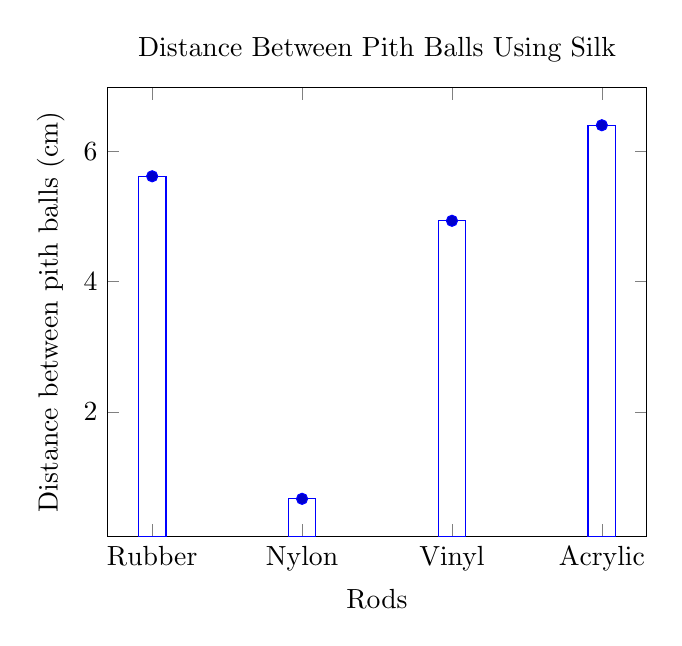
\begin{tikzpicture}
    \begin{axis}[
      title = {Distance Between Pith Balls Using Silk},
      symbolic x coords = {Rubber, Nylon, Vinyl, Acrylic},
      xtick = data,
      nodes near coords align={vertical},
      xlabel = {Rods},
      ylabel = {Distance between pith balls (cm)},
    ]
    \addplot+[ybar] plot coordinates
        {(Rubber,5.6166667) (Nylon, 0.6666667) (Vinyl,4.9333333) (Acrylic,6.4)};
    \end{axis}
  \end{tikzpicture}%
  \caption{}
\end{figure}

\begin{figure}[h!]
  \centering
  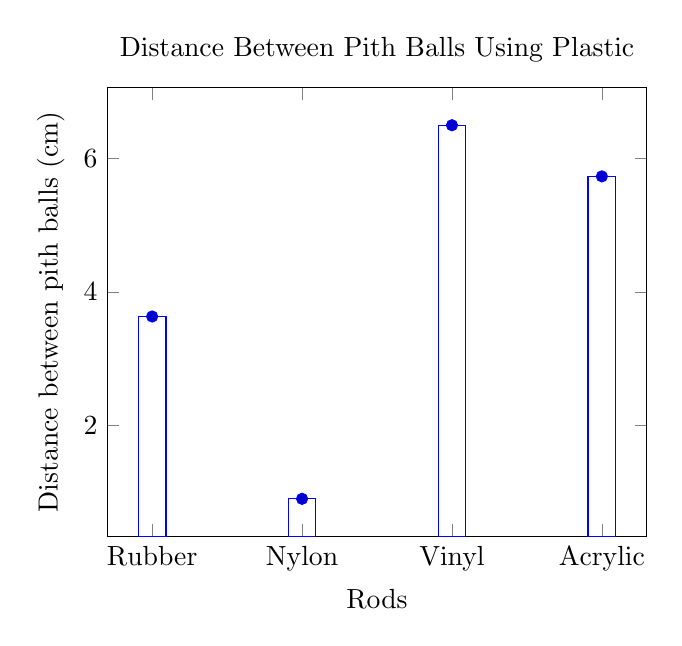
\begin{tikzpicture}
    \begin{axis}[
      title = {Distance Between Pith Balls Using Plastic},
      symbolic x coords = {Rubber, Nylon, Vinyl, Acrylic},
      xtick = data,
      nodes near coords align={vertical},
      xlabel = {Rods},
      ylabel = {Distance between pith balls (cm)},
    ]
    \addplot+[ybar] plot coordinates
        {(Rubber,3.6333333) (Nylon,0.9) (Vinyl,6.5) (Acrylic,5.7333333)};
    \end{axis}
  \end{tikzpicture}
  \caption{}
\end{figure}

\begin{figure}[h!]
  \centering
  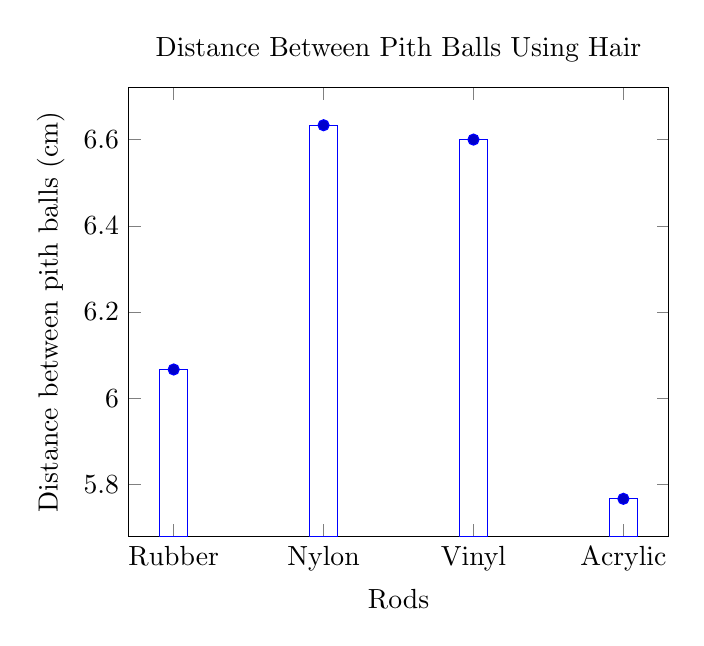
\begin{tikzpicture}
    \begin{axis}[
      title = {Distance Between Pith Balls Using Hair},
      symbolic x coords = {Rubber, Nylon, Vinyl, Acrylic},
      xtick = data,
      nodes near coords align={vertical},
      xlabel = {Rods},
      ylabel = {Distance between pith balls (cm)},
    ]
    \addplot+[ybar] plot coordinates
        {(Rubber,6.0666667) (Nylon,6.6333333) (Vinyl,6.6) (Acrylic,5.7666667)};
    \end{axis}
  \end{tikzpicture}
  \caption{}
\end{figure}

\begin{figure}[h!]
  \centering
  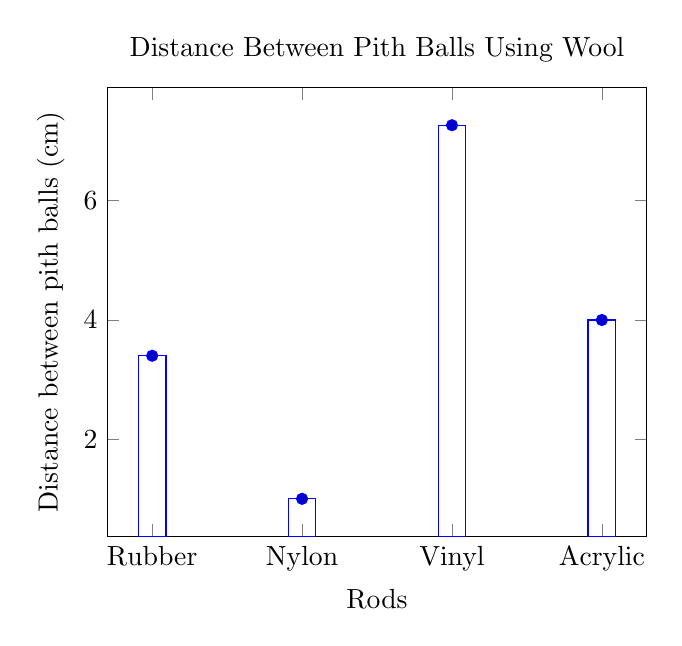
\begin{tikzpicture}
    \begin{axis}[
      title = {Distance Between Pith Balls Using Wool},
      symbolic x coords = {Rubber, Nylon, Vinyl, Acrylic},
      xtick = data,
      nodes near coords align={vertical},
      xlabel = {Rods},
      ylabel = {Distance between pith balls (cm)},
    ]
    \addplot+[ybar] plot coordinates
        {(Rubber,3.4) (Nylon,1) (Vinyl,7.2666667) (Acrylic,4)};
    \end{axis}
  \end{tikzpicture}
  \caption{}
\end{figure}

\pgfplotstableread{
X Y
0.056166667 0.000124169358 
0.006666667 0.0000140592135
0.064       0.00014365347
0.049333333 0.00010783345
0.036333333 0.0000780776033
0.009       0.0000189899857
0.057333333 0.000127016292
0.065       0.000146207576
0.060666667 0.000135253239
0.066333333 0.000149638717
0.057666667 0.000127833041
0.066       0.000148778135
0.034       0.0000728839413
0.01        0.0000211057941
0.04        0.0000863207909
0.072666667 0.000166368938
}\distanceAndForce

\begin {figure}
  \centering
  \begin{tikzpicture}
    \begin{axis}[
      title = {Distance Between Charges and Force of Charge},
      xlabel = {\(r\) (m)},
      ylabel = {\(F_{\text{charge}}\) (N)},
      ]
      \addplot [only marks, mark = *] table {\distanceAndForce};
      \addplot [thick, red] table[
        y={create col/linear regression={y=Y}}
      ]
      {\distanceAndForce};
    \end{axis}
  \end{tikzpicture}
  \caption {}
\end {figure}

\pgfplotstableread{
X Y
0.056166667 0.00000000659727543
0.006666667 0.000000000263492357
0.064       0.00000000808568429
0.049333333 0.00000000540002727

0.036333333 0.00000000338413143
0.009       0.000000000413412471
0.057333333 0.00000000681107479
0.065       0.00000000828470485

0.060666667 0.00000000743708455
0.066333333 0.000000000484261111
0.057666667 0.00000000391738668
0.066       0.00000000987984447

0.034       0.00000000305966295
0.01        0.000000000484261111
0.04        0.00000000391738668
0.072666667 0.00000000987984447
}\distanceAndCharge

\begin {figure}
  \centering
  \begin{tikzpicture}
    \begin{axis}[
      title = {Distance Between Charges and Charge Values},
      xlabel = {\(r\) (m)},
      ylabel = {\(q\) (C)},
      ]
      \addplot [only marks, mark = *] table {\distanceAndCharge};
      \addplot [thick, red] table[
        y={create col/linear regression={y=Y}}
      ]
      {\distanceAndCharge};
    \end{axis}
  \end{tikzpicture}
  \caption {}
\end {figure}

\subsection* {DISCUSSION OF RESULTS}
Figures 2 through 5 can be compared to what was expected for each rod/material combination. For instance, in Figure 2, it was expected that the acrylic rod would show the greatest distance between pith balls followed by vinyl, with nylon and rubber being equal. However, Figure 2 shows that while acrylic discharged the most, nylon and rubber did not behave as expected. \\\\
For plastic, it was expected that acrylic would show the greatest distance, followed by nylon, vinyl, and then rubber. The lowest, as shown in Figure 3, was nylon, which does not match expectations. \\\\
For hair, the expectation was for vinyl to discharge the greatest, followed by rubber, and equally, acrylic and nylon. However, nylon again disrupts expectations by having the greatest distance between the pith balls. Acrylic and rubber seem to follow expectations. \\\\
And lastly, for wool, vinyl was expected to show the greatest distance, followed by rubber, acrylic, and nylon. Figure 5 shows that these expectations were mostly met, with acrylic slightly exceeding the distance expected. \\

\subsection* {FURTHER STUDY}
The lab manual states that there are five materials to test (IIT, 3) and five rods to charge the pith balls with. The materials and rods presented at the lab station lacked both a mystery fur and a rayon rod, resulting in this epxeriment consisting of 16 rod/material combinations. Thus, if this experiment were to be repeated, the materials needed (see Equpiment) should be thoroughly checked. Since this experiment did not contain the full list, it is less rigorious than had it been executed in full. \\\\
Additionally, the value for the length of the string was not recorded during the experiment. The value implemented in this lab report was from a neighboring experiment, and as such, all representative material (tables and graphs) cannot fully model the actual experiment. \\\\
Care must be taken in order to outline the variables and materials needed in the future. 

\subsection* {SUPPLEMENTARY QUESTIONS}
1. Using the free-body diagrams of Figure 3, derive an expression for the charge in terms of the pith ball mass \emph{m}, and the separation distance “r”. \\\\
We know Coulomb's Law from Equation 1. The gravitational force for the pith balls is equal to the product of the mass and Earth's gravity constant. Using this information and the fact that the pith balls are not moving, the following is derived:
\begin{equation}
  \begin{split}
    F_{\text{charge}} &= F_{\text{tension}}\sin{\theta} \\
  \end{split}
\end{equation}

\noindent
Additionally:
\begin{equation}
  \begin{split}
    F_{\text{gravity}} &= F_{\text{tension}}\cos{\theta} \\
    m_{\text{ball}}g &= F_{\text{tension}}\cos{\theta} \\
  \end{split}
\end{equation}

\noindent
where \(\theta\) is the angle between the string and the vertical. The tension force can be solved for using the above Equation set 4:
\begin{equation}
  \begin{split}
    F_{\text{tension}} &= \dfrac{F_{\text{charge}}}{\sin{\theta}} \\
  \end{split}
\end{equation}

\noindent
Likewise, Equation set 5 can be used to solve for the tension force:
\begin{equation}
  \begin{split}
    F_{\text{tension}} &= \dfrac{m_{\text{ball}}g}{\cos{\theta}}
  \end{split}
\end{equation}

\noindent
Thus, since \(F_{\text{tension}}\) is solved for in Equation set 6 and 7, they can be combined:
\begin{equation}
  \begin{split}
    \dfrac{F_{\text{charge}}}{\sin{\theta}} &= \dfrac{m_{\text{ball}}g}{\cos{\theta}} \\
  \end{split}
\end{equation}

\noindent
To find \(F_{\text{charge}}\) in this experiment, \(F_{\text{charge}}\) can be solved for:
\begin{equation}
  \begin{split} 
    F_{\text{charge}} &= m_{\text{ball}}g\tan{\theta} \\
  \end{split}
\end{equation}

\noindent
To find \(q_{1}\) and \(q_{2}\), it must be known that these charges are equal, since they were equally charged by the rods. Thus, by substituting in Coulomb's Law (Equation 1), the charge on a pith ball, \(q\), can be solved for:
\begin{equation}
  \begin{split}
    k\dfrac{q_{1}q_{2}}{r^2} &= m_{\text{ball}}g\tan{\theta} \\
    k\dfrac{q^2}{r^2} &= m_{\text{ball}}g\tan{\theta} \\
    q &= \sqrt{\dfrac{r^{2}m_{\text{ball}}g\tan{\theta}}{k}} \\
  \end{split}
\end{equation}

\noindent
However, \(\theta\) was not measured. Using trig:

\begin{equation}
  \begin{split}
    \theta &= \sin^{-1}\left(\dfrac{r}{2l}\right) \\
  \end{split}
\end{equation}

\noindent
where \(l\) is the length of the string. Finally, Equation 10 can be combined with Equation 11 to calculate the charge force and charge on a pith ball using the mass of the ball and the length of the string. Below is how to calculate the charge force:

\begin{equation}
  \begin{split}
    F_{\text{charge}} &= m_{\text{ball}}g\tan{\theta} \\
    F_{\text{charge}} &= m_{\text{ball}}g\tan\left({\sin^{-1}\left(\dfrac{r}{2l}\right)}\right) \\
    F_{\text{charge}} &= m_{\text{ball}}g\left(\dfrac{r}{\sqrt{4l^2-r^2}}\right) \\
  \end{split}
\end{equation}

\noindent
Below is how to calculate the charge on a single pith ball:
\begin{equation}
  \begin{split}
    q &= \sqrt{\dfrac{r^{2}m_{\text{ball}}g\tan{\theta}}{k}} \\
    q &= \sqrt{\dfrac{r^{2}m_{\text{ball}}g\tan{\left(\sin^{-1}\left(\dfrac{r}{2l}\right)\right)}}{k}} \\
    q &= \sqrt{\dfrac{r^{2}m_{\text{ball}}g\left(\dfrac{r}{\sqrt{4l^2-r^2}}\right)}{k}} \\
    q &= \sqrt{\dfrac{r^{3}m_{\text{ball}}g}{k\sqrt{4l^2-r^2}}} \\
  \end{split}
\end{equation}

\noindent
2. Calculate the charge on the pith balls for each rod/soft material combination.  How many millions or billions of electrons reside on each pith ball? \\\\
An electron has a charge of about -1.60 \(\times 10^{-19}\) C (Boston University, "Electric charge and Coulomb's law"). Knowing this fact, the amount of electrons can be calculated for each pith ball in each combination of rod and material using the following:
\begin{equation}
  \begin{split}
    n &= \dfrac{q}{e} \\
  \end{split}
\end{equation}
where \(n\) is the number of electrons, \(q\) is the charge of one of the pith balls, and \(e\) is the charge of one electron.

\begin {table}[H]
  \centering
  \begin {tabular}{| c | c | c | c | c | c |}
    \hline\hline
    & & \multicolumn {4}{| c |}{Rods} \\
    \hline
    & & Rubber & Nylon & Acrylic & Vinyl \\
    \hline
    \multirow {4}{*}{Material} & Silk & 4.12 \(\times10^{10}\) & 1.65 \(\times10^{9}\) & 5.05 \(\times10^{-10}\) & 3.38\(\times 10^{10}\) \\ %329714 %682723 (LDR) %355268 %501704 (LDR)
    \cline{2-6}
    & Plastic & 2.12 \(\times10^{10}\) & 2.58\(\times10^{9}\) & 4.26 \(\times10^{10}\) & 5.18 \(\times10^{10}\) \\ %508214 (LDR) %382794 %692174 (LDR) %794053 (LDR)
    \cline{2-6}
    & Hair & 4.65\(\times 10^{10}\) & 5.35\(\times 10^{10}\) & 4.30\(\times 10^{10}\) & 5.30\(\times 10^{10}\) \\ %817784 (LDR) %579832 (LDR) %541544 (LDR) %361821
    \cline{2-6}
    & Wool & 1.91\(\times 10^{10}\) & 3.03\(\times10^{9}\) & 2.45\(\times 10^{10}\) & 6.17\(\times 10^{10}\) \\ %228934 %663194 (LDR) %836667 (LDR) %490279 (LDR)
    \hline\hline
  \end {tabular} \\
  \caption {Electrons in one pith ball (e)}
\end {table}

\noindent
3. Compare the extremely small gravitational attraction between the two pith balls with the repulsion of the electrostatic force. \\

\begin {table}[H]
  \centering
  \begin {tabular}{| c | c | c | c | c | c |}
    \hline\hline
    & & \multicolumn {4}{| c |}{Rods} \\
    \hline
    & & Rubber & Nylon & Acrylic & Vinyl \\
    \hline
    \multirow {4}{*}{Material} & Silk & 3.38 \(\times10^{-17}\) & 2.40\(\times 10^{-15}\) & 2.61 \(\times10^{-17}\) & 4.38 \(\times10^{-17}\) \\ %289494 %119976 %546875 (LDR) %495258
    \cline{2-6}
    & Plastic & 8.08 \(\times10^{-17}\) & 1.32 \(\times10^{-15}\) & 3.25 \(\times10^{-17}\) & 2.53 \(\times10^{-17}\) \\ %416815 %753086 (LDR) %661983 (LDR) %591716 (LDR)
    \cline{2-6}
    & Hair & 2.90 \(\times10^{-17}\) & 2.43 \(\times10^{-17}\) & 3.21 \(\times10^{-17}\) & 2.45 \(\times10^{-17}\) \\ %964977 (LDR) %539332 (LDR) %919506 (LDR) %995409 (LDR)
    \cline{2-6}
    & Wool & 9.23 \(\times10^{-17}\) & 1.07 \(\times10^{-15}\) & 6.67 \(\times10^{-17}\) & 2.02 \(\times10^{-17}\) \\ %183391 %72 (LDR) % %104198
    \hline\hline
  \end {tabular} \\
  \caption {Force of gravity between pith balls (N)}
\end {table}

\noindent
The proportion between the charge force and the gravitational force between the pith balls will be defined as:
\begin{equation}  
  \begin{split}
    \dfrac{F_{\text{charge}}}{F_{\text{gravitational}}} \\
  \end{split} 
\end{equation}

\noindent
Table 5 shows the proportion between the two forces for each rod/material pair.

\begin {table}[H]
  \centering
  \begin {tabular}{| c | c | c | c | c | c |}
    \hline\hline
    & & \multicolumn {4}{| c |}{Rods} \\
    \hline
    & & Rubber & Nylon & Acrylic & Vinyl \\
    \hline
    \multirow {4}{*}{Material} & Silk & 3.67 \(\times10^{12}\) & 5.86 \(\times10^{9}\) & 5.51 \(\times10^{12}\) & 2.46 \(\times10^{12}\) \\ %0505889 %5078671 (LDR) %353648 %9170265 (LDR)
    \cline{2-6}
    & Plastic & 9.66 \(\times10^{11}\) & 1.44 \(\times10^{10}\) & 3.91 \(\times10^{12}\) & 5.79 \(\times10^{12}\) \\ %8087493 (LDR) %1331378 %2262558 %8296557 (LDR)
    \cline{2-6}
    & Hair & 4.66 \(\times10^{12}\) & 6.17 \(\times10^{12}\) & 3.98 \(\times10^{12}\) & 6.07 \(\times10^{12}\) \\ %4468116 %966806 (LDR) %3336588 %2690734
    \cline{2-6}
    & Wool & 7.89 \(\times10^{11}\) & 1.98 \(\times10^{10}\) &1.29 \(\times10^{12}\) & 8.23 \(\times10^{12}\) \\ %4849714 %7679357 (LDR) %4164781 %1839796
    \hline\hline
  \end {tabular} \\
  \caption {Proportion of \(F_{\text{charge}}\) to \(F_{\text{gravitational}}\) (unitless)}
\end {table}

\noindent
4. Develop a way to determine if the mystery fur is from a rabbit or cat. If you have time, try your method out, to see if it works. If time is short, or humidity is too high, describe how one could carry out the method in conditions with lower humidity. \\\\ 
We know that the farther away two materials are in Figure 2 of the lab manual (IIT, 2), the greater affinity they have for receiving or depositing electrons. As such, we can determine whether the mystery fur is from a rabbit or a cat based on its combinations with the rods and the resulting distance. For rabbit fur, as we rub it with rods increasingly farther apart, the distance between the pith balls will increase. The order, from least to most distance for rabbit fur should be as follows: acrylic, nylon, plastic, rubber, and vinyl. For the cat fur, the order is as follows from least to most distance: nylon, acrylic and rubber, and vinyl.

\subsection* {REFERENCES}
Boston University. (n.d.). Electric charge and Coulomb's law. Retrieved February 5, 2020, from https://physics.bu.edu/~duffy/py106/Charge.html \\\\
Gladding, G., Selen, M. A., \& Stelzer, T. (2012). Electricity and Magnetism. New York: W.H. Freeman. \\\\
Illinois Institute of Technology. (n.d.). Experiment 1: Coulomb's Law. PDF. Chicago.
\end {document}
